\documentclass[a4paper,11pt]{article}

% Font
\usepackage[T1]{fontenc}
\usepackage[utf8]{inputenc}
\usepackage{lmodern}
\usepackage{tgbonum} % for extra boldness

% Graphics
\usepackage{graphicx}
\usepackage[usenames,pdftex,dvipsnames]{xcolor}
\usepackage{subcaption}

% Math
\usepackage{amsmath,amssymb,amsthm,textcomp}
\usepackage{enumerate}
\usepackage{multicol}
%\usepackage{tikz}

% Theorem / Proofs
\usepackage{amsthm}
\newtheorem{theorem}{Theorem}
\newtheorem*{remark}{Remark}

\usepackage{geometry}
\geometry{left=25mm,right=25mm,%
bindingoffset=0mm, top=20mm,bottom=20mm}
\linespread{1.3}

% Todo notes
\usepackage{xargs}
\usepackage[colorinlistoftodos,prependcaption,textsize=tiny]{todonotes}
\newcommandx{\unsure}[2][1=]{\todo[linecolor=red,backgroundcolor=red!25,bordercolor=red,#1]{#2}}
\newcommandx{\change}[2][1=]{\todo[linecolor=blue,backgroundcolor=blue!25,bordercolor=blue,#1]{#2}}
\newcommandx{\info}[2][1=]{\todo[linecolor=OliveGreen,backgroundcolor=OliveGreen!25,bordercolor=OliveGreen,#1]{#2}}
\newcommandx{\inlineinfo}[2][1=]{\todo[inline,linecolor=OliveGreen,backgroundcolor=OliveGreen!25,bordercolor=OliveGreen,#1]{#2}}
\newcommandx{\improvement}[2][1=]{\todo[linecolor=Plum,backgroundcolor=Plum!25,bordercolor=Plum,#1]{#2}}
\newcommandx{\thiswillnotshow}[2][1=]{\todo[disable,#1]{#2}}

% my own titles
\makeatletter
\renewcommand{\maketitle}{
  \begin{center}
    \vspace{2ex}
    {\huge \textsc{\@title}}
    \vspace{1ex}
    \\
    \@author \hfill \@date
    \vspace{4ex}
  \end{center}
}
\makeatother
%%%

% custom footers and headers
\usepackage{fancyhdr}
\pagestyle{fancy}
\lhead{}
\chead{}
\rhead{}
\lfoot{GeomLab 2020}
\cfoot{}
\rfoot{Page \thepage}
\renewcommand{\headrulewidth}{0pt}
\renewcommand{\footrulewidth}{0pt}
%

% code listing settings
\usepackage{listings}
\lstset{
  language=Python,
  basicstyle=\ttfamily\small,
  aboveskip={1.0\baselineskip},
  belowskip={1.0\baselineskip},
  columns=fixed,
  extendedchars=true,
  breaklines=true,
  tabsize=4,
  prebreak=\raisebox{0ex}[0ex][0ex]{\ensuremath{\hookleftarrow}},
  frame=lines,
  showtabs=false,
  showspaces=false,
  showstringspaces=false,
  keywordstyle=\color[rgb]{0.627,0.126,0.941},
  commentstyle=\color[rgb]{0.133,0.545,0.133},
  stringstyle=\color[rgb]{01,0,0},
  numbers=left,
  numberstyle=\small,
  stepnumber=1,
  numbersep=10pt,
  captionpos=t,
  escapeinside={\%*}{*)}
}

% No paragraph indentation
\setlength{\parindent}{0in}

% ----------------------
\begin{document}
% ----------------------

\title{GeomLab 2020}
\author{}
\date{\today}
\maketitle

% ----------------------
\tableofcontents
% ----------------------

\newpage

% ----------------------
\section{Motivation}
% ----------------------

Motivated by the COVID-19 disease several outlets printed two-dimensional depictions of data which usually contained multidimensional datasets. These datasets usually compromise \{\textit{infections, recoverd, death}\} rates with regard to the \textit{country} and sometimes also the evolution over \textit{time}.\\

\begin{figure}[h]
  \begin{subfigure}{0.5\textwidth}
    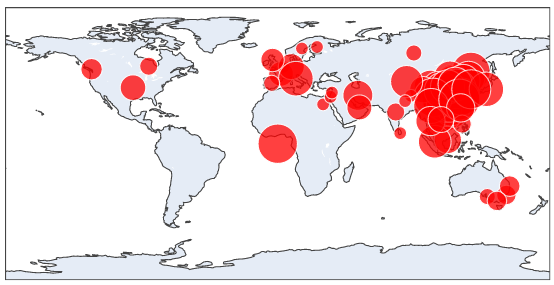
\includegraphics[width=0.9\linewidth]{covid_spread_20200223.png}
    \caption{23.02.2020}\label{fig:covid2020Feb}
  \end{subfigure}
  \begin{subfigure}{0.5\textwidth}
    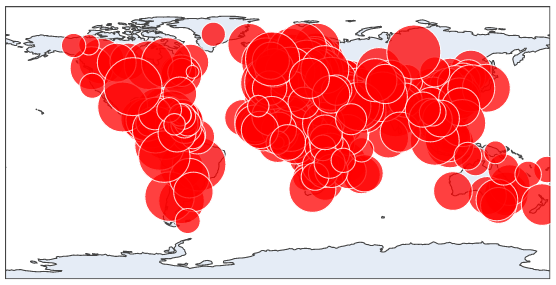
\includegraphics[width=0.9\linewidth]{covid_spread_20200511.png}
    \caption{11.05.2020}\label{fig:covid2020May}
  \end{subfigure}
  \caption{Comparison of a typical scatterplot depicting the $log$ of confirmed cases as the radius.}
  \label{fig:covid19}
\end{figure}

In this lab we focus on depicting data in a meaningful way. Besides its quantitative nature this task has some qualitative properties. Similar to many solutions of problems in computational geometry, like deciding if a point is contained in a polygon or the construction of a convex hull for a set of points, the quality of the scatterplot is obvious to the human observer. Not so for a machine. While Fig. (\ref{fig:covid2020Feb}) is highly informative for a human or potential policy maker, Fig. (\ref{fig:covid2020May}) bears little information content. Despite this fact both figures result from the very same algorithm depicting data from the disease spread of COVID-19 during 2020 [Algo im Appendix].\\

To investigate the quantification of visual quality mainly Tufte in 1983 in \textit{The visual display of quantitative information graphics press"} and Miller et al in \textit{The Need For Metrics In Visual Information Analysis} provided fundamental work. Based on this, follow-up work and further considerations from visibility problems and sorting we develop a novel approach to visualize multidimensional data in a scatterplot which transports as much information content as possible.\\
Our main resource will be the Paper by Sergio Vabello at al \textit{Algorithmic Aspects of Proportional Symbol Maps}. In this Paper the hardness of maximizing utility measures with regards to physically realizable drawings was discussed and another type of drawing given by a stacking order was defined. For those drawings some algorithms which we will briefly discuss were derived. Those algorithms where derived for proportional Symbol Maps which only allow us to depict a single quantity. We will try to find more general glyphs and use slightly adapted algorithms to get optimal result with regards to those glyphs. Our many focus will be nested Circles, centered nested Circles and Pie Charts. 
\newpage

% ----------------------
\section{Problem Statement}
% ----------------------
Sergio Vabello at al discussed proportional Symbol maps. For those we have $n$ circles in $R^2$ and the radius or size of the circles corresponds to some quantity which is associated to the center point of the circle. The problem is to find a drawing which retains as much of the information about the quantity and the location of the center as possible. \\
For the definition of a drawing they describe two approaches. One is given by physically realizable drawings. \color{blue} Hier müsste dann diese Definition noch beschrieben werden. \color{black}\\
The other far simpler one is a stacking order which is given by a bijection $\phi: [n]\rightarrow [n]$. This bijection describes the order in which the circles are drawn. Circles which are drawn later cover parts over the circles which are drawn earlier. Therefore our task is to find a stacking order such that as little as possible of every circle is covered. \\
Now we need to discuss what we mean by covering as little as possible. We want that the viewer of the map should be able to judge the size of the Circles and the center point. We could try to maximize the area of the circles which is not covered, but there are cases in which that would not allow the viewer to get all of the information. The approach we will use is to maximize the visible boundary of our Glyph. We can define the visible and occluded boundary for circles formally by 
\begin{align*}
U_i^{vis}&=\partial C_i\textbackslash \bigcup_{\phi(j)>\phi(i)} C_{j}\\
U_i^{occ}&=\partial C_i \cap \bigcup_{\phi(j)>\phi(i)} C_{j}.\\
\end{align*}
Some results which are given in \textit{Algorithmic Aspects of Proportional Symbol Maps} are the following
\begin{theorem}
It is NP-hard to decide if a given collection of congruent disks has a
physically realizable drawing where at least some given length of the perimeter of
each disk is visible
\end{theorem}
This implies that trying to maximize the minimal $U_i^{vis}$ with respect to physically realizable drawings is NP-hard.
\begin{theorem}
It is NP-hard to decide if a given collection of disks has a physically
realizable drawing whose total visible perimeter is at least a given value.
\end{theorem}
This implies that trying to maximize the sum over all the $U_i^{vis}$ with respect to physically realizable drawings is NP-hard.\\
For stacking orders they give a positive result with regards to the minimum:
\begin{theorem}
Given n disks in the plane, a stacking order maximizing the boundary
length of the disk that is least visible can be computed in $O(n^2 \log n)$ time.
\end{theorem} 
If a polynomial algorithm for the sum of all the $U_i^{vis}$ exists remains open.
\\ 

We won't try to construct an algorithm for the sum problem. Instead we will be looking at glyphs which can depict more information. The first glyph we will discuss are nested Disks. Formally every Glyph $G^i$ is given by a set of circles $G^i_1,...,G^i_k$ such that $r_{j+1}>r_j$ and $G^i_{j+1}\subset G^i_j$ for all $j\in \{1,...,k-1 \}$. Often times figures using nested disks also center all the discs in the same point. The second type of glyphs we will use are pie charts. A pie chart is formally given by a circle $C_i$ and a set $\{\alpha_1^i,...\alpha_k^i\}$ of dividing lines which we can encode as angle in $[0,2\pi ]$.\\
In the next section we will be discussing an easy general approach for maximizing special Utility functions for Glyph stacking order drawings and then apply it to our glyphs and some utility functions.


\section{Stacking order algorithms for more general Glyphs}
We will be focusing on utility functions which follow the following formula: Maximize the local utility of the worst glyph. In the example of the disk glyphs the local utility would just be the visible perimeter. \\We can use a simple greedy algorithm to solve the problem. At each time step just calculate for all discs their visible perimeter if they were the bottommost disk and then choose the disc $C_i$ with the largest visible perimeter and then draw it. In the next timestep we look at the set of disks without $C_i$. This is done until we have processed all disks.\\
We can now formalize this approach for more general objects and prove that the greedy algorithm is optimal with respect to the utility.
\\

Let $D$ be a finite set and for $d \in D$ and $S \subseteq D$ the function $ \Gamma(d, S) \mapsto \Re_{\geq 0} $ with the property, that for every $d \in D$ we have $S' \subseteq S => \Gamma(d, S') \geq \Gamma(d, S)$. \\
The set $D$ corresponds to our set of glyphs and $\Gamma$ corresponds to a utility function, which depends on the insertion order, i.e the set $S$ describes all the glyphs which lie above d. Let $\phi: \{1,...,n\} \mapsto D$ be a stacking order. Then the for every glyph $d_i:=\phi(i)$ the set of glyphs above $d_i$ is given by $\{d_j\ \in D | j > i\}$.

\begin{figure}[!t]
\begin{lstlisting}[mathescape=true ]
ALG(finite set $D$) 
  $x := \text{argmax}_{d \in D} \Gamma(d, D \setminus {d})$
  return [$x$, ALG($D \setminus {x}$)]
\end{lstlisting}
\caption{The greedy algorithm}
\end{figure}

\begin{theorem}
For a given set $D$ and a local utility function $\Gamma$ the greedy Algorithm as described in Figure 2 returns a stacking order which maximizes\begin{align*}
\min_{d_i \in D} \Gamma(d_i, \{d_j\ \in D | j > i\}).
\end{align*} 
\end{theorem}
\begin{proof}
\color{blue}
existiert muss noch getext werden
\color{black}
\end{proof}
We can use this theorem for object of any kind. In particular for the glyphs we discussed before. We now only need to define some reasonable utility functions for our different glyphs and calculate them locally with reasonable run-time.

\subsection{Centered nested disks}
For centered nested disks we can easily define local Utility measures. Every Glyph $G$ corresponds to $k$ nested circles therefore we could just calculate the visible perimeter for the $k$ circles and then just combine them by choosing the minimum of the $k$ circles or the the sum of the visible perimeter of the $k$ circles. For some set $S$ of objects above $G_i$ we then get formally:
\begin{align*}
\Gamma_{min}({G^i,S})=\min_j  {^{vis} G^i_j}\\
\Gamma_{sum}({G^i,S})=\sum_{j=1}^k  {^{vis} G^i_j}
\end{align*} 
We may also be interested in the relative Utility which is given by normalizing the size of the circles. This relative approach stops the small circles from dominating big circles. In our applications there is close to no different between the relative utility and the normal one. \\
For $\Gamma_{min}$ it may happen that for all glyphs the smallest circle may be completely covered. Then the Utility would be zero for all of the circles. If that happens the algorithm has an optimal solution of value zero. If that happens, we perform the greedy step again and ignore the smallest circle in all of the glyphs until we get a value bigger than zero. This heuristic gives better results than just choosing a random circle.\\
\begin{remark}
It is NP-hard to calculate physically realizable drawing where $\min\Gamma_{min}$ or $\min\Gamma_{sum}$ is maximized since disc glyphs are a special case of nested discs and both utility measures coincide and are equal to the visible circumference.
\end{remark}

\subsection{Nested disks}
For dense Regions centered nested discs loose a lot of information since the small circles can easily be completely covered up. Therefore we will now derive an algorithm which guaranties, that every nested circle is at least visible. To achieve that we will allow the circles to be moved inside each other. We still want to have $r_{j+1}>r_j$ and $G^i_{j+1}\subset G^i_j$ for all $j$ but the centers can be different.\\
Our approach is quite simple. We first just look at the biggest circle of each glyph. For those we perform our greedy algorithm with the local utility given by the size of the maximal \textbf{continuous} visible perimeter. After we have done that we can take the point $p$ on the circle which is in the middle of the continuous visible perimeter piece and connect it to the center of the big circle by a line. Now every center point for a nested inner circle is uniquely defined by positioning it on that line such that the circle touches the point $p$. The final glyphs look a little bit like the \textit{Hawaiian earring} topological space.\\
The resulting drawing guarantees that the perimeter of every circle is at least a little bit visible. The downside of this construction is that the drawing look a little bit strange to the viewer and its more difficult to focus the center of a glyph.




\subsection{Pie charts}


\newpage

% ----------------------
\section{Experimental validation}
% ----------------------

\begin{figure}[htp]
  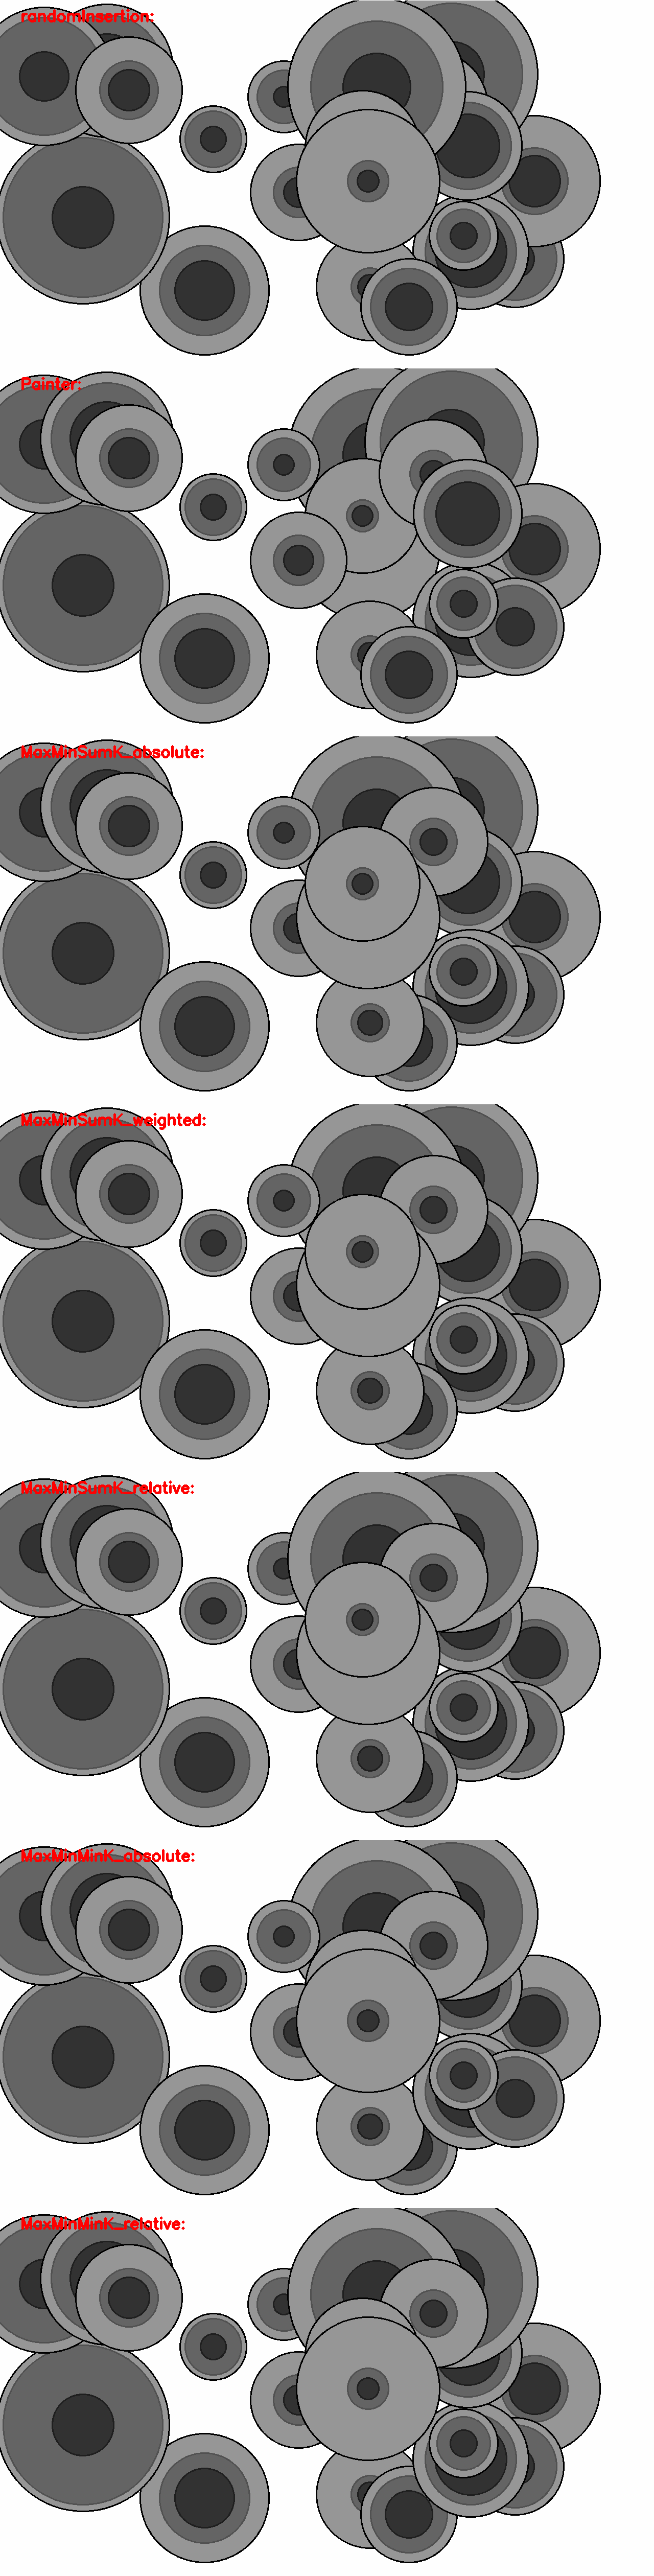
\includegraphics[width=\textwidth,height=0.7\textheight,keepaspectratio]{assets/cost_functions.png}
\end{figure}

\begin{figure}[htp]
  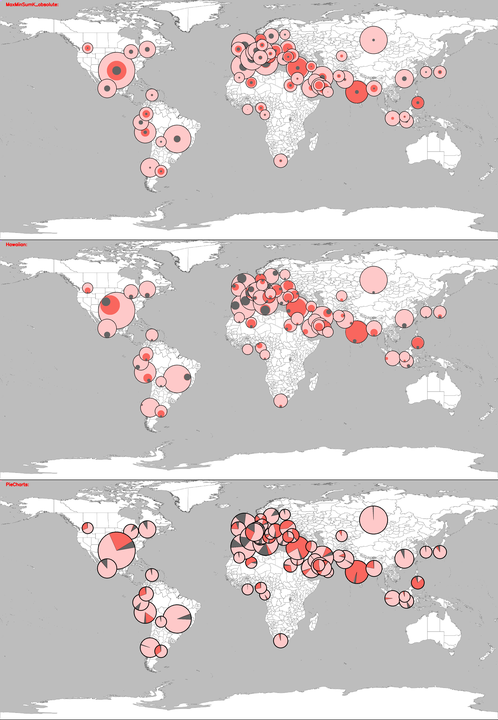
\includegraphics[width=\textwidth,height=\textheight,keepaspectratio]{assets/covid19_nested_discs.png}
\end{figure}

\begin{figure}[htp]
  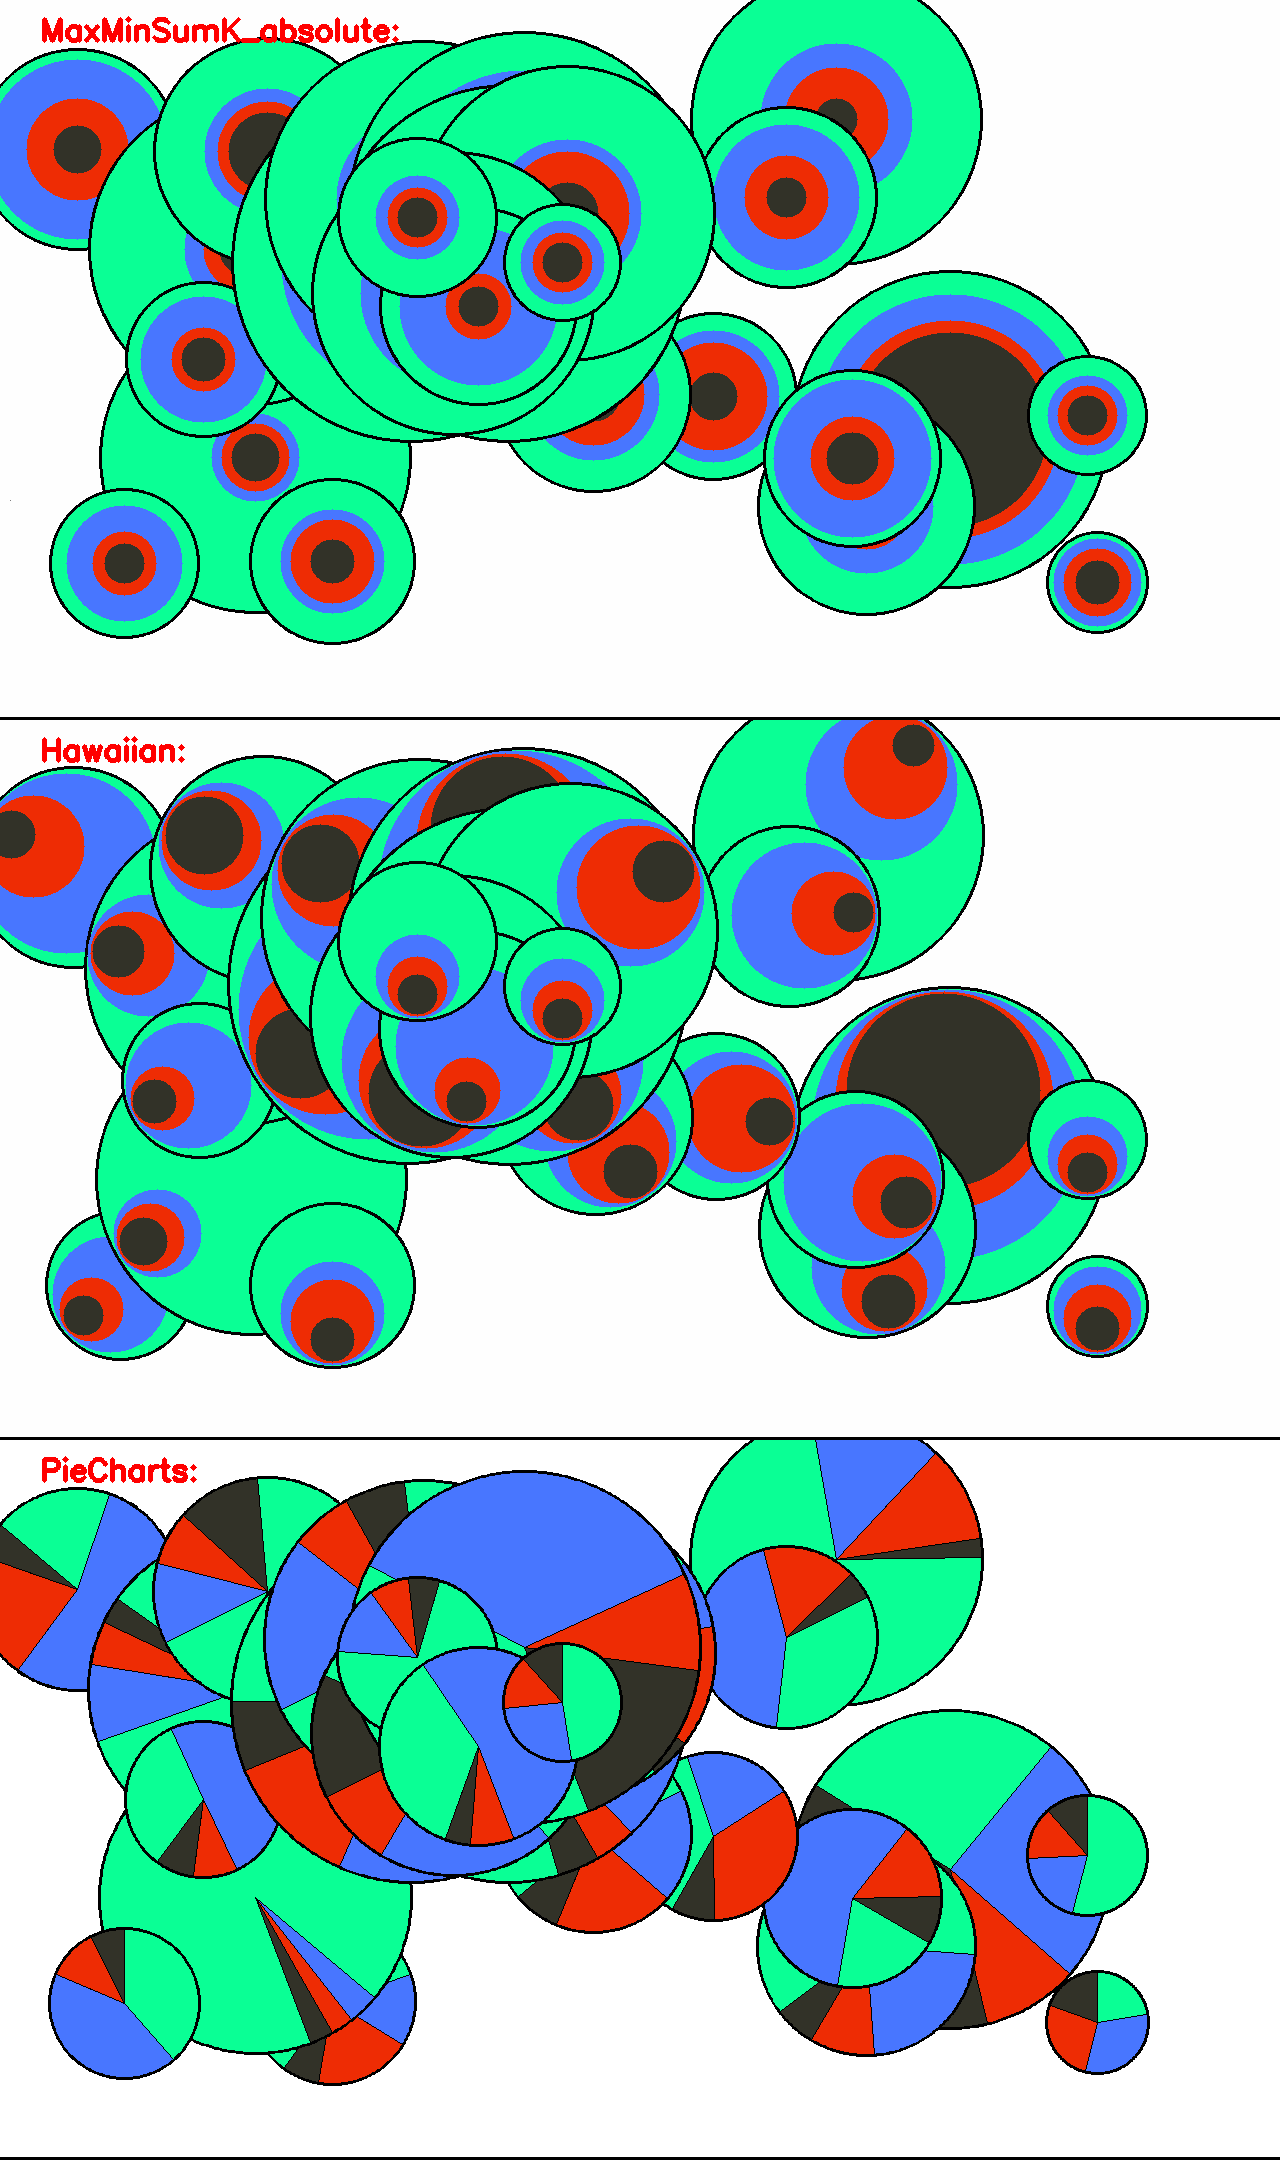
\includegraphics[width=\textwidth,height=\textheight,keepaspectratio]{assets/nested_discs_all.png}
\end{figure}

\newpage


\section{Sources}


Tufte, Edward R. "The visual display of quantitative information graphics press." Cheshire, Connecticut (1983).\\

Miller, Nancy, et al. "The need for metrics in visual information analysis." Proceedings of the 1997 workshop on New paradigms in information visualization and manipulation. 1997.\\

Brath, Richard. "Metrics for effective information visualization." Proceedings of VIZ'97: Visualization Conference, Information Visualization Symposium and Parallel Rendering Symposium. IEEE, 1997.\\

Tatu, Andrada, et al. "Visual quality metrics and human perception: an initial study on 2D projections of large multidimensional data." Proceedings of the International Conference on Advanced Visual Interfaces. 2010.\\

Urribarri, D. K., \& Castro, S. M. (2016). Prediction of data visibility in two-dimensional scatterplots. Information Visualization, 16(2), 113–125. doi:10.1177/1473871616638892\\

Coeurjolly, D., Miguet, S., \& Tougne, L. (2004). 2D and 3D visibility in discrete geometry: an application to discrete geodesic paths. Pattern Recognition Letters, 25(5), 561–570. doi:10.1016/j.patrec.2003.12.002\\

Yang-Pelaez J and Flowers WC. Information content
measures of visual displays. In: Proceedings of the IEEE symposium on information vizualization 2000 (INFOVIS’00), 2000, pp. 99–103. Washington, DC: IEEE Computer Society.


\end{document}

\begin{enumerate}
  \item Information content covered by the data,
  \item information content of the data in the visualization,
  \item information capacity of a visualization,
  \item topological information content.
\end{enumerate}

\begin{enumerate}
  \item Random inseration
  \item Painter
  \item MaxMinSumK/absolute - Sum of visible circumference/hull
  \item MaxMinSumK/weighted - weighted such that big circles/glyphs not dominate
  \item MaxMinSumK/relative - Sum of relative circumference/hull
  \item MaxMinMinK/absolute - MaxMin of minimal visible circumference/hull of each circle/glyph
  \item MaxMinMinK/relative
\end{enumerate}


Let $D$ be a finite set and for $d \in D$ and $S \subseteq D$ the function $ \phi(d, S) \mapsto \Re_{\geq 0} $ with the property, that for every $d \in D$ $S' \subseteq S => \phi(d, S') \geq \phi(d, S)$.

Let the stacking-order $\pi: \{1,...,n\} \mapsto D$ be bijective.


  
The algorithm

\begin{verbatim}
ALG(finite set D) {
  x := argmax_{d \in D} \phi(d, D \setminus {d})
  return [x, ALG(D \setminus {x})]
}
\end{verbatim}

returns a stacking-order, which maximizes $min_{d \in D} \phi(d, \{d\ \in D | d' > d\})$.

\unsure{Roland: shouldn't it be 'minimizes'?}

\begin{proof}
  Given an optimal stacking-order $s$ and output of ALG $s^*$ .

  \begin{enumerate}
    \item case: $s=s^*$. Done.
    \item case: $s \neq s^*$. $s \neq s^*$ implies, that there is a lowest $k \in N$, such that $s(k) \neq s^*(k)$. Let $s(k) = d_k$ and $s^* = d^*_k$. Hence, $k^* = s^{-1}(s^*(k)) = s^{-1}(d^*_k)$ is the index of $d^*_k$ with respect to $s$. It follows $k<k^*$.

    We modify $s$ such, that at point in time\unsure{Roland: point in 'time'? It's an order so it would be 'at position' as far as I see.}, we insert disc $d^*_k$ and shift all others towards the end. Let this new stacking-order be $s'$.
    \inlineinfo{Roland: What end, small or large end?}

    Comparing $s$ and $s'$, we find that $s'$ selects all discs later. That means, that all $\phi$-values are at least bigger. 

    Now $d^*_k$ is chosen in $s'$, as well as in $s^*$ at position $k$.\unsure{Roland: Argumentiere hier mit Position. Das macht mEn mehr Sinn. Warte auf Eure Kommentare.} As $d^*_k$ was chosen by $s^*$, $d^*_k$ has to maxmize $\phi$. Therefore, it is bigger or equal to $d_k$, as $s$ and $s^*$ are identical except at position $k$.

  \end{enumerate}
\end{proof}

\begin{remark}
  $\phi$ may be the visible glyph boundary, the visible glyph boundary, the visible surface or the distance of...\unsure{Roland: Proof stops.}
\end{remark}


\begin{enumerate}
  \item Rotation
  \item Physics/Heuristics based approaches
\end{enumerate}

\begin{figure}[htp]
  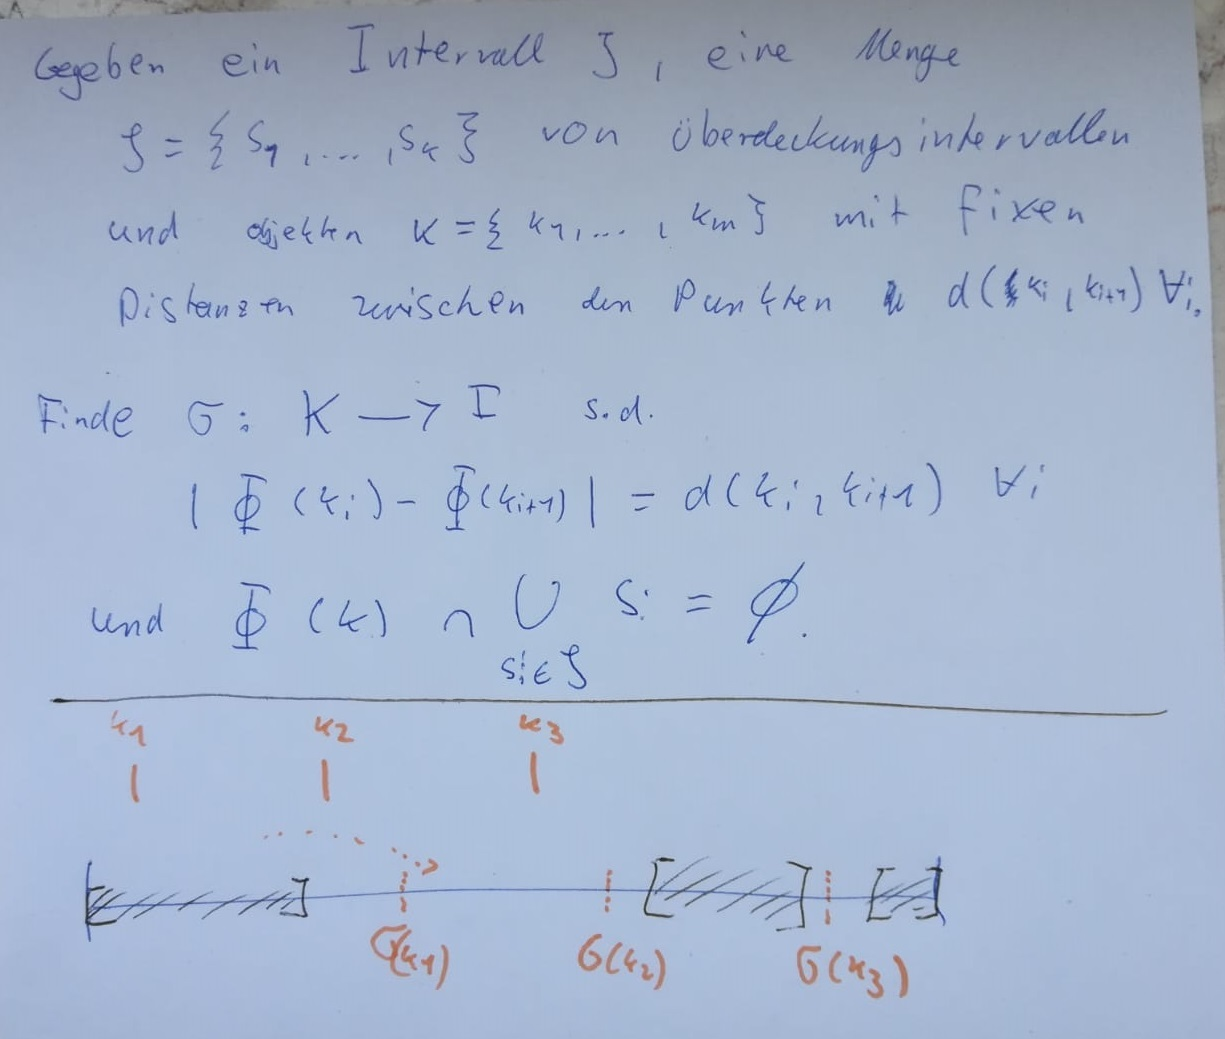
\includegraphics[width=\textwidth,height=\textheight,keepaspectratio]{assets/trennlinienproblem.jpg}
  \caption{Trennlinienproblem}
\end{figure}




% code from http://rosettacode.org/wiki/Fibonacci_sequence#Python
\begin{lstlisting}[label={list:first},caption=Sample Python code -- Fibonacci sequence calculated analytically.]
from math import *

# define function 
def analytic_fibonacci(n):
  sqrt_5 = sqrt(5);
  p = (1 + sqrt_5) / 2;
  q = 1/p;
  return int( (p**n + q**n) / sqrt_5 + 0.5 )

# define range
for i in range(1,31):
  print analytic_fibonacci(i)
\end{lstlisting}

Following Listing~\ref{list:first}\ldots{} 

Tufte proposed to measure quality based on the amount of consumed ink and purpose of the ink. He stated that the majority of the used ink in a graph must represent information about the data. Most recently Tatu et al. showed "that quality measures can simulate the selection of best views by human beings." and also compares a set of promising and established measures. In the motivated usecase, especially scatterplots using glyphs like circles or discs are of major interest, because of their advantages when plotting multidimensional data [Tatu et al.].\\

In a first step, following the common depiction, we consider circles as glyph. Further, we assume that the data $\mathcal{D}$ is finite and three-dimensional. We map two dimensions to the location $(x_i, y_i)$ and the remaining one dimension of our data set to the radius $r_i$ of a circle $C_i$, i.e., $ (x_i, y_i, r_i) \in \mathcal{D} \subset \mathbb{R}^3$. Moreover, we ignore transparency and other means to circumvent the occlusion of circles overlaying each other.\\

As already mentioned in the Motivation we want to maximize visibility of the data. Urribari et al define visibility as
%
\begin{equation} \label{eq1}
  \begin{split}
    visiblity & = 1 - occlusion \\
              & = f(data(set), visualization \, parameters)\\
  \end{split}
\end{equation}
%
with $occlusion$ being defined as [Tatu et al.]:
%
\begin{equation}
  occlusion = { \text{no. of data points completely occluded } \over \text{total no. of data points}}\\
\end{equation}

Using this simple definition it is possible to formulate two equivalent cost functions already now:
%
\begin{equation} \label{eq3}
  \begin{split}
    \min\limits_{\text{vis. par.}} & \; occlusion\\
    \max\limits_{\text{vis. par.}} & \; visiblity\\
  \end{split}
\end{equation}
%
We focus on visiblity for now. When using circles as glyphs, we can split the visibilty in two components:
%
\begin{equation} \label{eq3}
  \begin{split}
    U_i = & \delta C_i \, \setminus \bigcup_{D} C_j\\
    A_i = & \, C_i \; \setminus \bigcup_{D} C_j\\
  \end{split}
\end{equation}
%
and sum over the visible circumferences and areas
%
\begin{equation} \label{eq3}
  \begin{split}
    U_{occlusion} & = \sum_i U_i\\
    A_{occlusion} & = \sum_i A_i\\
  \end{split}
\end{equation}
%
which already hints toward potential cost functions.\\

Here many variations and specific options are thinkable. Like considering (1) relative circumference to circle area, (2) relative area to circumference, etc.
